\documentclass{beamer}
%Information to be included in the title page:
\title{Pénzváltás probléma}
\author{Polonkai Dávid (GPNWZT)}
\institute{Miskolci Egyetem}
\date{2022}

\begin{document}

\frame{\titlepage}

\begin{frame}
\frametitle{Pénzváltás probléma}
\begin{itemize}
    \item Egy pénzösszeget milyen módon tudunk elérni kisebb címletekből?
    \item Hátizsák feladat speciális esete
    \item Dinamikus programozással megoldható (részekre bontás)
\end{itemize}

\end{frame}
\begin{frame}
    \frametitle{Hátizsák feladat}
    \textbf{Túrázni megyünk. Miket vigyünk a túrára a hátizsákunkba?}
    Legyen \(n\) a lehetséges tárgyak száma. \newline
    \(B\) a teherbírásunk. \newline
    Legyen \(a_1,a_2,...,a_n\) a tárgyak súlya.\newline
    Legyen \(c_1,c_2,...,c_n\) a tárgyak értéke (hasznossága)\newline
    \(x_j\) (0 vagy 1), a \(j\). tárgyat a hátizsákba helyezzük vagy sem.\newline  
    Feltételek:  
    \[\sum_{j=1}^{n}c_j x_j \rightarrow max\]
    \[\sum_{j=1}^{n}a_j x_j \le B\]
    Tehát a nálunk található tárgyak a lehető leghasznosabbak legyenek, de a tömegük ne haladja meg a teherbírásunkat.
\end{frame}
\begin{frame}
    \frametitle{Pénzváltás probléma}
    \textbf{Egy pénzösszeget akarunk pontosan kifizetni egy adott pénzrendszer címleteivel úgy,
    hogy minimális számú pénzdarabot használunk fel.}\\
    \(n\) a pénzrendszer címleteinek a száma.\\
    Legyen \(a_1,a_2,...,a_n\) az egyes címletek értékei.\newline
    Legyen \(B\) a kifizetendő összeg.\newline
    \(x_j\) egész szám a \(j\) címelet darabszámát mutatja.\newline  
    Feltételek:  
    \[\sum_{j=1}^{n}x_j \rightarrow min\]
    \[\sum_{j=1}^{n}a_j x_j = B\]
    Tehát a lehető legkevesebb címlettel fizessük ki a B összeget.
\end{frame}
\begin{frame}
    \frametitle{Pénzváltás probléma}
    \textbf{Létezik-e megoldás?}  \newline
    \(A = \{a_1,a_2,...,a_n\}\) a címletek halmaza.\newline
    \(b\) egy pozitív egész szám.\newline
    \(\sum_{a \in S} = B\), ahol \(S \subseteq A\).\newline
    Megjegyzés: a címletek csak egyszer használhatóak fel, tehát \(x_j\) 0 vagy 1 lehet, és tetszőleges egész számok lehetnek.\newline
\end{frame}
\begin{frame}
    \frametitle{Létezik-e megoldás}
    Egy megoldás:
    \[B = a_{i_1} + \dots + a_{i_k}, i_1 < ... <i_k\] \newline
    Ekkor 
    \[B-a_{i_k} = a_{i_1} + \dots + a_{i_{k-1}}\]
    megoldása lesz annak a feladatnak, amelyben a felváltandó érték: \(B-a_{i_k}\),
     felváltásához legfeljebb \((a_1,...,a_{i_{k-1}})\) címleteket használhatjuk.
\end{frame}
\begin{frame}
    \frametitle{Részproblémákra bontás}
    Minden \((X,i)\) \((1 \leq X \leq B, 1 \leq i \leq n)\)számpárra,
    \(X\) felváltható-e az első \(a_1,...,a_i\) pénzzel. \newline
    \(V(X,i) = Igaz\), ha az első \(i\) pénzzel előállítható.   \newline
    \(V(X,i) = Hamis\), ha az első \(i\) pénzzel nem állíható elő.
\end{frame}
\begin{frame}
    \frametitle{Részproblémák eredménye (Rekurzív megoldás)}
    \[
        V(X,i) \Leftrightarrow
    \begin{cases}
        X=a_i\vee &&
        i>1\wedge V(X,i-1)\vee&&
        i>1\wedge >a_i\wedge V(X-a_i,i-1)&&
    \end{cases}
    \]
\end{frame}
\begin{frame}
    \frametitle{Részproblémák eredménye (Táblázatos módszer)}
    Kiszámítási sorrend módosítása, hogy először azokat számoljuk ki, amelyek szükségesek
    a későbbi számításokhoz. \newline
    \((X,i)\) probléma összetevői: \((X,i-1)\) és \((X-a_i,i-1)\) \newline
    Ezért a következő táblázatot soronként alulról felfele, balról jobbra töltjük ki.
\end{frame}
\begin{frame}
    \frametitle{Táblázat}
    \centering
    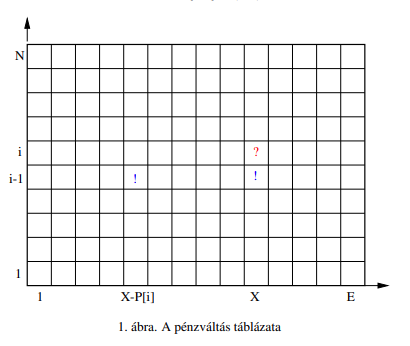
\includegraphics[scale=0.6]{table.png}
\end{frame}
\begin{frame}
    \frametitle{A Pénzváltás probléma, egy felváltás eloállítása}
    Megoldás csak akkor létezhet, ha az aktuális problémára nézve \(V[B,n]=Igaz\). \newline
    Keressük azt a legkisebb \(i\) értéket, amelyre \(V[B,i]=Igaz\), tehát $V[B,i-1]=Hamis$. \newline
    Ebből tujuk, hogy \(a_i\) pénz szerepel a \(B\)-ben.\newline
    Folytatva ezt a folyamatot \(B-a_i\)-re és \(i-1\)-re,\\ azaz $V[B-a_i,i-1]$-re addig, amíg $B=0$-t nem kapunk.
\end{frame}
\begin{frame}
    \frametitle{Optimális pénzváltás}
    Az előző diában bemutatott mohó stratégia nem optimális, mivel 8 = 5+1+1+1 eredményt adna.\newline
    Az optimális megoldáshoz a már előzőleg bevezetett részproblémákra bontást alkalmazzuk.\newline
    Minden \((X,i)\) \((1 \leq X \leq B, 1 \leq i \leq n)\) számpárra,\newline
    legkevesebb hány pénz összegeként lehet az \(X\)-et előállítani \newline
    legfeljebb az első \(i\{a_1,\dots,a_i\}\) pénz felhasználásával.
    Ha nincs megoldás, akkor legyen \(n+1\).\newline
    A probléma optimális megoldása: \(Opt(X,i)\)
    Az optimális megoldás értéke: \(X=0\)-ra és \(i=0\)-ra, \(Opt(X,0)=n+1\) és \(Opt(0,i)=0\).
    Mindezek alapján az alábbi rekurzív összefüggés írható fel
\end{frame}
\begin{frame}
    \frametitle{Optimális pénzváltás}
    \[
        Opt(X,i) =
    \begin{cases}
        \infty & \text{ha } i=0\wedge X>0 \\
        0 &\text{ha} X=0 \\
        Opt(X,i-1)& \text{ha} X<a_i \\
        min(Opt(X,i-1),\\1+Opt(X-a_i,i-1))& \text{ha} X \ge a_i
    \end{cases}
    \]
\end{frame}
\begin{frame}
    \frametitle{Optimális pénzváltás}
    Az előző rekurzív kifejezést, színtén táblázatba tudjuk foglalni, mivel $Opt(X,i)$-nek legfeljebb $Opt(X-a_i,i-1)$-re vagy $Opt(X,i-1)$-re van szüksége.\\
    A táblázatból a felváltás előállítását, a már bemutatott módszer módosításával hajthatjuk végre.
\end{frame}
\begin{frame}
    \frametitle{Optimális pénzváltás, egy optimális felváltás előállítása}
    Megoldás csak akkor létezhet, ha az aktuális problémára nézve \(V[B,n]<\infty\). \newline
    Keressük azt a legkisebb \(i\) értéket, amelyre \(V[B,i]\rightarrow min\), tehát $V[B,i-1]>V[B,i]$ (hiszen $a_i>a_{i-1}$). \newline
    Ebből tujuk, hogy \(a_i\) pénz szerepel a \(B\) optimális felváltásában.\newline
    Folytatva ezt a folyamatot \(B-a_i\)-re és \(i-1\)-re,\\ azaz $V[B-a_i,i-1]$-re addig, amíg $B=0$-t nem kapunk.
\end{frame}
\begin{frame}
    
    Megoldás csak akkor létezhet, ha az aktuális problémára nézve \(V[B,n]<\infty\). \newline
    Keressük azt a legkisebb \(i\) értéket, amelyre \(V[B,i]\rightarrow min\), tehát $V[B,i-1]>V[B,i]$ (hiszen $a_i>a_{i-1}$). \newline
    Ebből tujuk, hogy \(a_i\) pénz szerepel a \(B\) optimális felváltásában.\newline
    Folytatva ezt a folyamatot \(B-a_i\)-re és \(i-1\)-re,\\ azaz $V[B-a_i,i-1]$-re addig, amíg $B=0$-t nem kapunk.
\end{frame}
\begin{frame}
    \frametitle{Felhasznált irodalmak}
    1. Horváth Gyula Szegedi Tudományegyetem Természettudományi és Informatikai Kar Algoritmizálás jegyzet\\
    2. Dr. Házy Attila: Nemlineáris optimalizálás. (elektronikus jegyzet)\\
    3. J. W. Wright. 1975. The Change-Making Problem. J. ACM 22, 1 (Jan. 1975), 125–128. https://doi.org/10.1145/321864.321874\\
\end{frame}
\begin{frame}
    \textbf{KÖSZÖNÖM A FIGYELMET!}
\end{frame}
\end{document}